\chapter{Introduction}

Program verification is a field in computer science that aims to mathematically prove the \emph{correctness} of software.
Correctness, in this context, meaning that a program's behavior satisfies a given specification under a defined set of assumptions.
For example, verifying a sorting algorithm involves proving that it genuinely produces a non-decreasing sequence, that all initial elements are preserved in the result, and that no additional elements are introduced.
Program correctness is particularly critical in scenarios where software failure could endanger lives or result in significant economic loss.
While traditional testing provides assurance regarding specific known scenarios, it cannot exhaustively rule out forgotten edge cases.
Formal verification is valuable precisely because it allows us to rule out entire classes of erroneous behaviors rather than just isolated instances.
Although programs can be verified using manual mathematical proofs, such a process is tedious, labor-intensive, and prone to human error.
Consequently, there are increasing efforts to mechanize and automate the verification process using specialized software tools.
% TODO ref?


\section{Translational Program Verifiers}

One way to build such tools is using \emph{translational} program verifiers.
They take a higher-level specification or language
and translate it into a lower-level language with simpler specifications.
This process operates analogously to a compiler. % TODO ref
For instance, just as a C++ compiler takes a program written in C++, translates it into LLVM IR, and finally compiles it into x86 assembly,
a translational verifier breaks down complex programmatic specifications into simpler logical assertions and assumptions.

For verification, one might take a practical programming language, such as Python,
and instrument it with specified pre- and postconditions.
A tool like Nagini\footnote{\url{https://www.pm.inf.ethz.ch/research/nagini.html}}
can then take the instrumented Python program as input and produce an equivalent program in Viper
\footnote{\url{https://www.pm.inf.ethz.ch/research/viper.html}}.
Viper is an Intermediate Verification Language (IVL) that helps mitigate the task of building a custom verification tool
for every programming language by handling the core verification logic that is shared across languages.
This is similar to how LLVM simplifies building a compiler by providing a unified target language before assembly. 

Viper programs may then\footnote{Viper also offers an alternative verification backend using symbolic execution.} be translated into another IVL called Boogie\footnote{\url{https://github.com/boogie-org/boogie}}.
These Boogie programs are ultimately translated into Verification Conditions (VCs)
formulated in the SMT format\footnote{\url{https://smt-lib.org/}}, which is a standardized way to represent mathematical formulas.
These VCs can then be checked by an SMT solver, such as Z3\footnote{\url{https://www.microsoft.com/en-us/research/project/z3-3/}}.
Another prominent IVL that targets Boogie as its backend is Dafny\footnote{\url{https://dafny.org/}}.


% \begin{figure}[t]
%   \centering
%   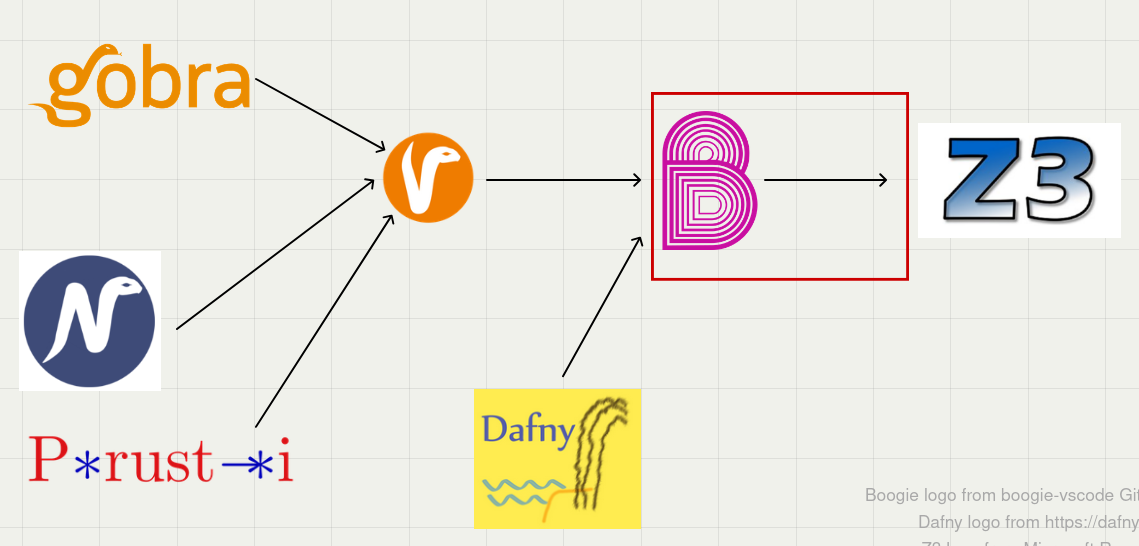
\includegraphics[width=0.95\textwidth]{uploads/verification-pipeline.png}
%   \caption{[TODO replace Screenshot with better diagram] Example verification pipeline for translational verifiers. Front-end tools such as Nagini, Prusti, and Gobra translate programs into intermediate verification languages such as Viper and Boogie, while Dafny targets Boogie directly. The resulting verification conditions are then discharged by an SMT solver such as Z3.}
%   \label{fig:verification-pipeline}
% \end{figure}


\section{Motivation}
\label{sec:motivation}

The ultimate goal of program verification is to guarantee the correctness of a program.
To achieve this, we must verify not only the input programs but also the verification tools themselves.
While there exist theoretical justifications for why certain verification approaches are sound,
there are seldom formal guarantees about their actual software implementations.
Ideally, we want a mechanism to prove that if the output of a translation is verifiable,
then the input program is guaranteed to be correct as well.
Providing these foundational guarantees is the primary goal behind the Viper Roots project
\footnote{\url{https://www.pm.inf.ethz.ch/research/roots.html}}.

There has been significant prior work in this space by Parthasarathy et al.~\cite{parthasarathy2021formally}, 
specifically targeting the Boogie-to-SMT segment of the verification pipeline.
Their approach certifies specific runs of the verifier by generating a machine-checked proof demonstrating that the validity of the SMT output implies the correctness of the Boogie input.
We explain the relevant components of this architecture in more detail in Section~\ref{sec:prior-work}.

The prior work established an immense foundation for certifying this translation.
Unfortunately, it currently only supports a restricted subset of the Boogie language.
Our goal is to extend this support to more complex features,
especially those heavily used by front-end IVLs such as Viper and Dafny,
so they can be fully integrated into the certification pipeline.
Expanding the supported subset to cover a broader range of real-world Boogie programs forms the core motivation for this project.


\section{Contributions}

This project makes the following contributions:

\paragraph{Updating the Codebase} The previous iteration of the certification pipeline was based on an outdated version of Boogie.
We updated the architecture and proof generation module to be compatible with a newer release.

\paragraph{Identifying the usage of Boogie by Dafny} We analyzed which missing Boogie features Dafny relies on most heavily in order to prioritize the next features for formalization.

\paragraph{Map Semantics} We designed and implemented formal semantics for Boogie maps that successfully support a practical subset of use cases.

\paragraph{Proof Generation} We implemented rudimentary proof automation and generation capable of certifying Boogie programs that use maps. 
This serves as a successful proof of concept for our approach, which we evaluated against a suite of custom test cases.


\section{Outline}
The remainder of this report is structured as follows.
Section~\ref{sec:background} introduces the relevant components of the prior work, the Boogie IVL,
and other foundational technologies used in this project, such as the Isabelle/HOL interactive theorem prover. 
Section~\ref{sec:upgrading-boogie} details how we updated the codebase and outlines the necessary architectural changes. 
In Section~\ref{sec:unsupported-usage}, we justify our decision to formalize Boogie maps and explain how we chose which specific behaviors to support. 
Section~\ref{sec:support-boogie-maps} presents the main contribution of this project:
the design of the formal semantics for Boogie maps, alongside an explanation of
how the proof generation module was adjusted to provide initial support for this feature. 
Section~\ref{sec:discussion} evaluates the successes of the project,
discusses current limitations, explores alternative approaches, and outlines avenues for future work. 
Finally, Section~\ref{sec:conclusion} concludes the thesis.
